\documentclass[border = 1cm, preview, varwidth = \maxdimen]{standalone}

\usepackage{xeCJK}
\usepackage{ifthen}

% mathematics
\usepackage{amsmath}
\usepackage{amssymb}
\usepackage{derivative}
\derivset{\pdif}[style-notation=multiple]
\usepackage{esint}

% tikz
\usepackage{tikz}
\usepackage{tikz-cd}
\usetikzlibrary{arrows}
\usetikzlibrary{automata}
\usetikzlibrary{positioning}
\usetikzlibrary{shapes}
\tikzset{
  ->, > = stealth', node distance = 1in,
  failure/.style = {dashed},
  state/.style = {ellipse, draw, minimum size = 1cm},
}

\begin{document}

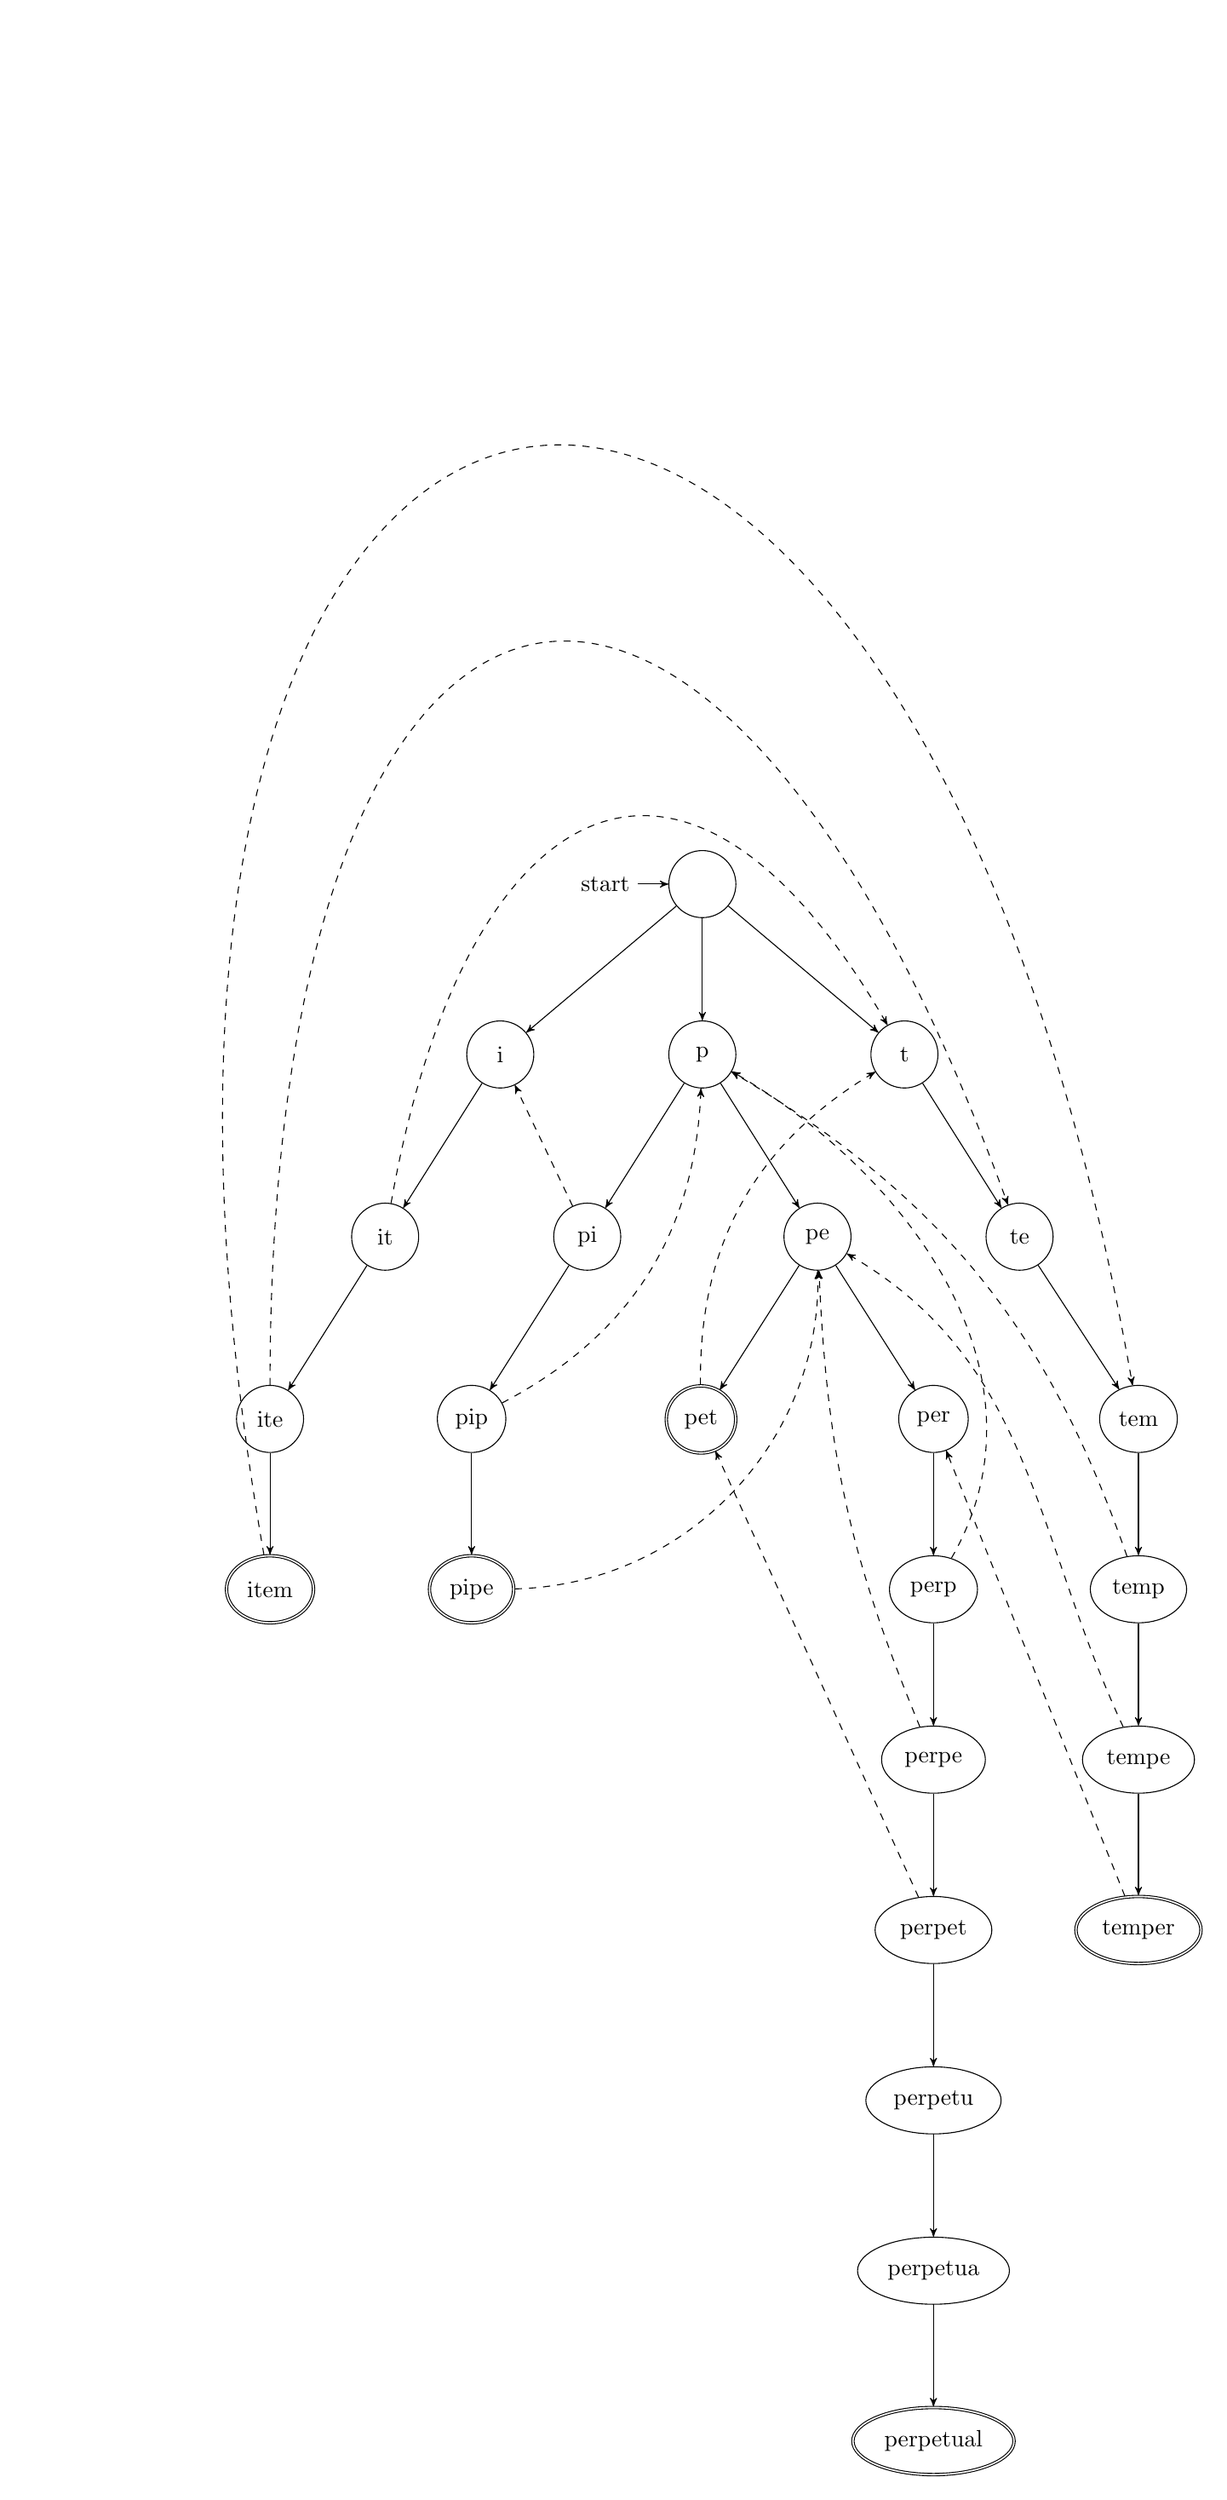
\begin{tikzpicture}
  % nodes
  \node [state, initial] (root) {};
  \node [state, below of = root] (p) {p};
  \node [state, right = 2 of p] (t) {t};
  \node [state, left = 2 of p] (i) {i};
  \node [state, below left = 2cm and 1cm of p] (pi) {pi};
  \node [state, below right = 2cm and 1cm of p] (pe) {pe};
  \node [state, below left = 2cm and 1cm of i] (it) {it};
  \node [state, below right = 2cm and 1cm of t] (te) {te};
  \node [state, below left = 2cm and 1cm of it] (ite) {ite};
  \node [state, below left = 2cm and 1cm of pi] (pip) {pip};
  \node [state, accepting, below left = 2cm and 1cm of pe] (pet) {pet};
  \node [state, below right = 2cm and 1cm of pe] (per) {per};
  \node [state, below right = 2cm and 1cm of te] (tem) {tem};
  \node [state, accepting, below of = ite] (item) {item};
  \node [state, below of = tem] (temp) {temp};
  \node [state, accepting, below of = pip] (pipe) {pipe};
  \node [state, below of = per] (perp) {perp};
  \node [state, below of = temp] (tempe) {tempe};
  \node [state, below of = perp] (perpe) {perpe};
  \node [state, accepting, below of = tempe] (temper) {temper};
  \node [state, below of = perpe] (perpet) {perpet};
  \node [state, below of = perpet] (perpetu) {perpetu};
  \node [state, below of = perpetu] (perpetua) {perpetua};
  \node [state, accepting, below of = perpetua] (perpetual) {perpetual};
  % edges
  \draw (root) -- (i);
  \draw (root) -- (t);
  \draw (root) -- (p);
  \draw (i) -- (it);
  \draw (t) -- (te);
  \draw (p) -- (pe);
  \draw (p) -- (pi);
  \draw (it) -- (ite);
  \draw (te) -- (tem);
  \draw (pi) -- (pip);
  \draw (pe) -- (pet);
  \draw (pe) -- (per);
  \draw (ite) -- (item);
  \draw (pip) -- (pipe);
  \draw (per) -- (perp);
  \draw (tem) -- (temp);
  \draw (perp) -- (perpe);
  \draw (temp) -- (tempe);
  \draw (perpe) -- (perpet);
  \draw (tempe) -- (temper);
  \draw (perpet) -- (perpetu);
  \draw (perpetu) -- (perpetua);
  \draw (perpetua) -- (perpetual);

  \draw [failure, out = 80, in = 120, looseness = 2] (it) to (t);
  \draw [failure, out = 90, in = 110, looseness = 3] (ite) to (te);
  \draw [failure, out = 100, in = 100, looseness = 4] (item) to (tem);
  \draw [failure, out = 60, in = 330] (perp) to (p);
  \draw [failure, bend left = 10] (perpe) to (pe);
  \draw [failure] (perpet) to (pet);
  \draw [failure, bend left] (pet) to (t);
  \draw [failure] (pi) to (i);
  \draw [failure, bend right] (pip) to (p);
  \draw [failure, bend right = 45] (pipe) to (pe);
  \draw [failure, bend right = 20] (temp) to (p);
  \draw [failure, out = 115, in = 330] (tempe) to (pe);
  \draw [failure] (temper) to (per);
\end{tikzpicture}

\end{document}
